\subsection{Elasticity in 1D}
\renewcommand{\arraystretch}{2.2}
	\begin{tabularx}{ \columnwidth} {p{3cm}XlX}
		\hline 
		\multicolumn{4}{p{\columnwidth}}{Stored momentum sets an object into motion. If the object doesn't move, but a momentum is applied, the object deforms.}\\
		Hook's Law & $F = k\cdot \Delta u$ &
		momentum   & $p = m\cdot v$\\
		
		momentum flux & $J_p = \dfrac{\partial p}{\partial t}$&
		momentum flux density & $j_p = \dfrac{J_p}{A}$\\
		
		mechanical stress (Spannung) & $\sigma_{11} = -j_p = \frac{-J_p}{A} $ &
		cutting force, flux of momentum & $F = \int_A \sigma_{11} dA$\\
		mechanical strain (Elastizität) &$\varepsilon_{11} = \dfrac{\partial u(x)}{\partial x}$&
		Youngs Modulus (Eleastizitätsmodul) &  $E = \dfrac{\sigma_{11}}{\varepsilon_{11}} $\\		
		Young Modulus & $F = \dfrac{EA_0\Delta L}{L_0}$&&\\
		\hline 
		\textbf{Momentum Balance equation} & $\dfrac{\partial \sigma_{11}}{\partial x} + \rho g= 0$ &
		boundary cond. & $\sigma_{11}(0) = \dfrac{F}{A} \newline  \sigma_{11}(L) = 0$ \\
		
		Displacement Field & $u(x) = \Delta u \cdot \dfrac{x}{L}$ & 
		$u(L) = \Delta x$ &  u(0) = 0 \\
		Material Law & $\varepsilon_{11}$\newline $ E $\\ 
		
	\end{tabularx}
\renewcommand{\arraystretch}{1.2}	
	 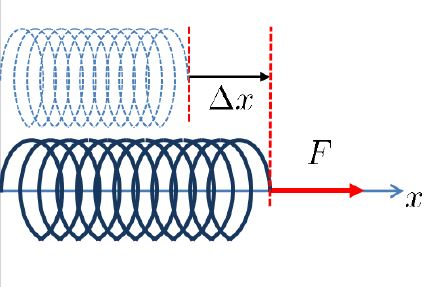
\includegraphics[scale = 0.3]{images/hook}
		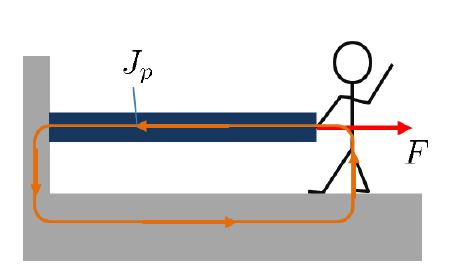
\includegraphics[scale=.3]{images/momentcons}
		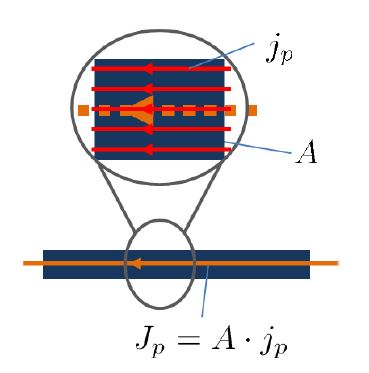
\includegraphics[scale=.3]{images/momflux}
		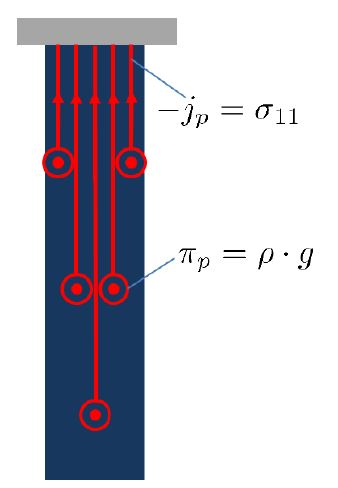
\includegraphics[scale=.3]{images/momfluxdensity}
		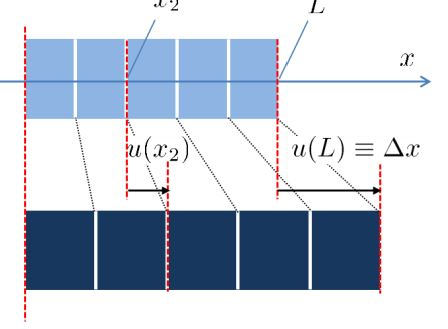
\includegraphics[scale=.3]{images/strain}
%		\includegraphics[scale=.3]{images/}				


\begin{tabularx}{\columnwidth}{p{3cm}XX}
	\hline 
	\multicolumn{3}{c}{Elasticity in a hanging rope}\\
	\hline 
	\multicolumn{3}{l}{The Rope is hanging from the ceiling in the gravitational Field of the earth}\\
	
	measured values& $L, A,\rho, E, g$ & \\
	mechanical stress & $\dfrac{\partial \sigma}{\partial x}  + \rho g = 0 \qquad \sigma(x) = -\rho g x + C$ & $\sigma(0) = \dfrac{F}{A} = \dfrac{mg}{A} = \dfrac{mgL}{AL} = L\rho g$\\
	&$\sigma(0) =\rho g L \qquad \sigma(x)  = \rho g(L-x)$ &
	$\sigma(x) = \varepsilon(x) E = \dfrac{\partial u(x)}{\partial x}E = \rho g(L-x)$\\
	strain & $\varepsilon(x)= \dfrac{\rho g}{E}(L-x)$ & $u(x) = \int \varepsilon(x)dx = \dfrac{\rho g}{E}(Lx-\dfrac{x^2}{2}+C)$\\
	Displacement Field& $u(0) = 0 \quad u(x) =\dfrac{\rho g}{E}(Lx-\dfrac{x^2}{2})$ & \\
	maximal stress & $\sigma_{max} = \rho g L$ \hspace{1.3cm}maximal elongation&  $\dfrac{\partial u}{\partial x} = 0 \Rightarrow  x_{max} = L \quad u_{max} = \dfrac{\rho g}{2E}L^2$\\

	\hline 
	\multicolumn{3}{c}{calculating a spring constant}\\
	\hline 
	measured values & $L, A, E$&\\
	& $\sigma = \dfrac{F}{A} = \text{const} \quad u(x) = \dfrac{F}{AE}x$ & elongation for $x=L \quad \Delta u = \dfrac{FL}{AE}$\\
	spring const. & $F = k\cdot \Delta u$ & $k = \dfrac{AE}{L}$\\
	\hline 
	
\end{tabularx}
\newpage

\subsection{Elasticity in 3D}
	electrodyamics: scalar charge $q$ $\Rightarrow$ vectorial flux $j$ (0 rank tensor $\Rightarrow$ 1st rank tensor)
	
	mechanics: vector momentum $\mathbf{p}$ $\Rightarrow$ tensorial flux density $\mathbf{\sigma}$ (1st rank tensor $\Rightarrow$ 2nd rank tensor)

%	$$
%	\sigma = \begin{pmatrix}
%	\sigma_{11} & \sigma_{12} & \sigma_{13} \\
%	\sigma_{21} & \sigma_{22} & \sigma_{23} \\
%	\sigma_{31} & \sigma_{32} & \sigma_{33} 
%	\end{pmatrix}
%	$$

\begin{tabularx}{ \columnwidth} {p{4cm}lX}
	\hline 
	General momentum balance equation &  $\dfrac{\partial \sigma_{ik}}{\partial x_k} + \rho g_i = 0$ & $\sigma_{ij}$: stress tensor of 2nd rank, characterizes material symmetry: $\sigma_{ij} = \sigma_{ji}$\\
	Cutting Force & $F_i^\alpha = \sigma_{ik} nA^\alpha_k \cdot A^\alpha$ & $\mathbf{n}^\alpha$: normal vector pointing outside of the cuboide\newline $A^\alpha$: face area 
	\\
	
	Angular Momentum &
	$\mathbf{M} = 0 $ &
	\\
	Stress Decomposition &  $\sigma^{iso}=\frac{\operatorname{tr} \sigma}{3} \cdot \mathbb{I} \equiv \frac{1}{3} \mathbb{E} : \varepsilon$ 
	&$\sigma^{shear}= \left(\mathbb{I}- \frac{1}{3}\mathbb{E} \right) : \varepsilon\qquad $ 
	$\sigma^{shear} = \sigma -\sigma^{iso}$\\ 
	
	$\begin{pmatrix}
	x\to x & x\to y & x\to z \\
	y\to x & y\to y & y\to z \\
	z\to x & z\to y & z\to z \\		
	\end{pmatrix}$&
	\multicolumn{2}{l}{\vspace{0cm}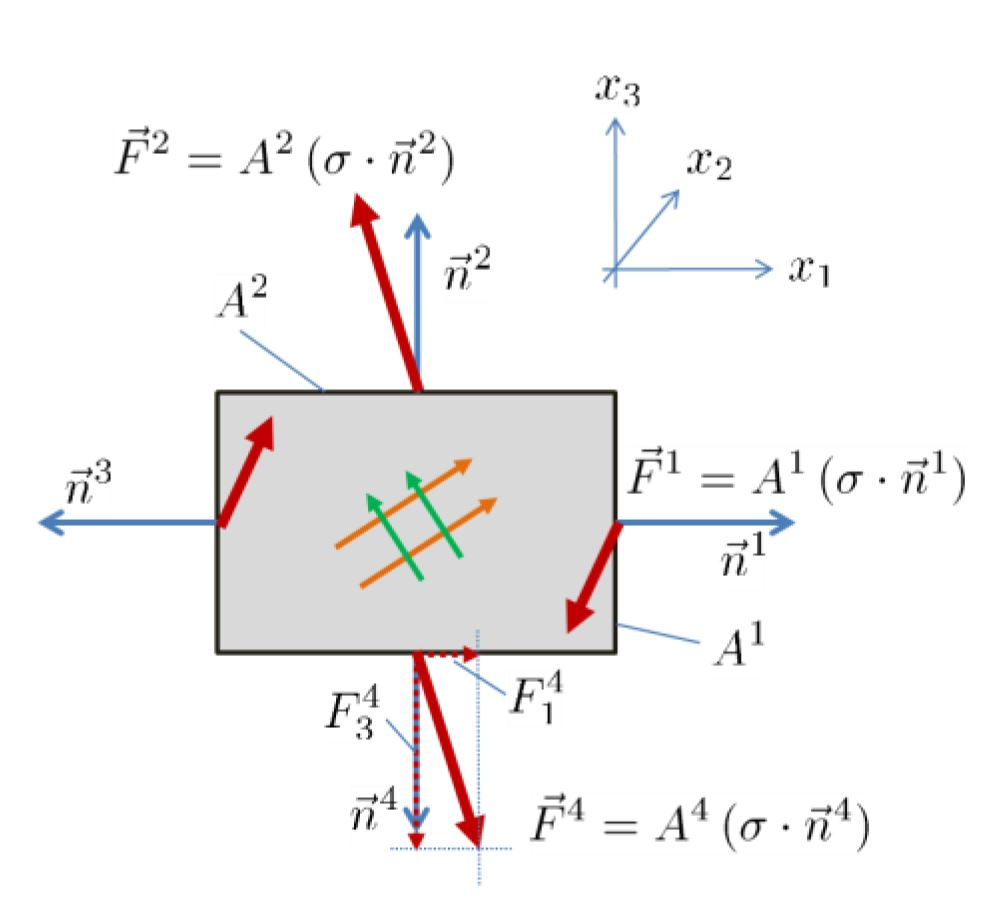
\includegraphics[scale=.15]{images/3Dcuttingforces} 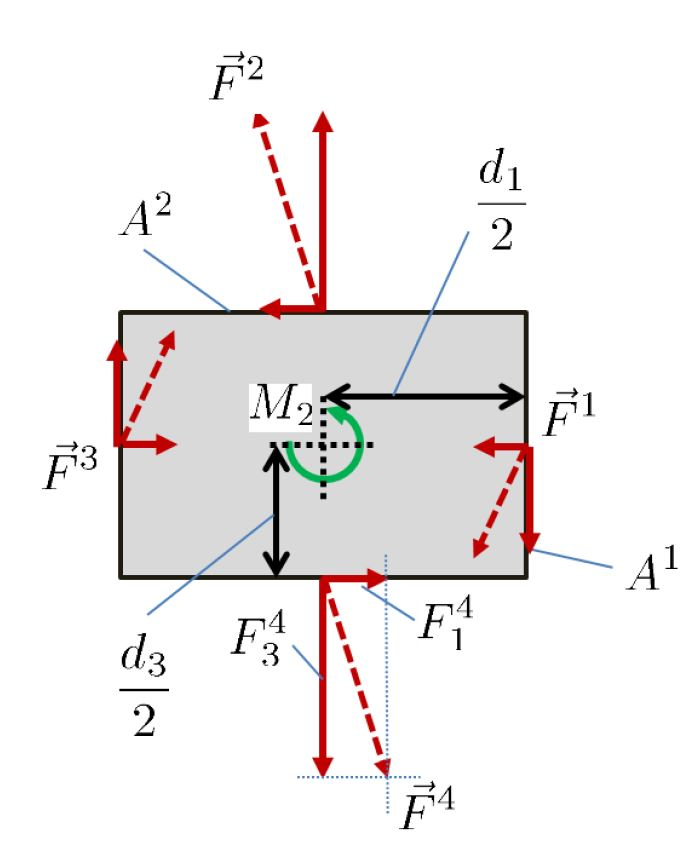
\includegraphics[scale=.15]{images/3Dangularmomentum}}	\\
	\hline 
\end{tabularx}
	\renewcommand{\arraystretch}{2}
\subsection{Special Stress States (Mechanische Spannung $\sigma = F/A$)}
	\begin{tabularx}{\columnwidth}{p{2cm}p{2cm}XX}
		\hline 
		Stress State & Tensor law & matrix notation & \\ 
		\hline 
		Isotropic Stress State & $\sigma_{ij} = -P\delta_{ik}$&	$ \sigma = \begin{pmatrix} -P & 0 & 0\\ 0 & -P & 0\\ 0 & 0 & -P \end{pmatrix}$ &\vspace*{-1.2cm}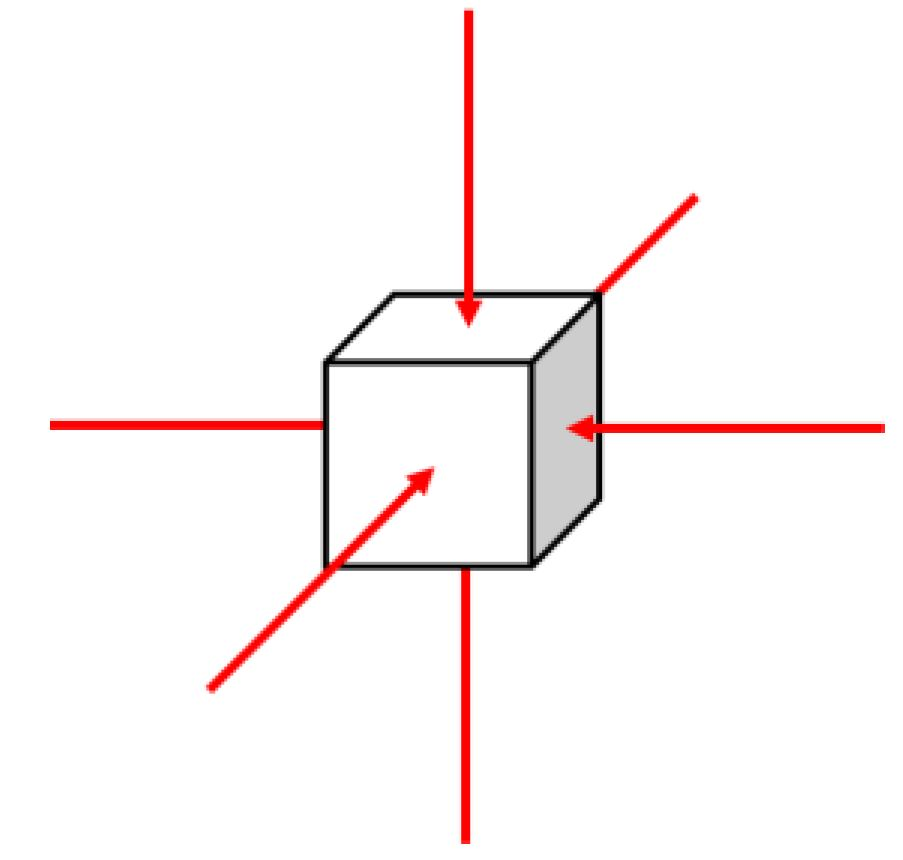
\includegraphics[scale=.11]{images/3Dcfisotropic}\\
		\hline 
		Uniaxial Stress State & & 		$ \sigma = \begin{pmatrix} \sigma_{11} & 0 & 0\\ 0 & 0 & 0\\ 0 & 0 & 0\\ \end{pmatrix}$ &		\vspace*{-1.2cm}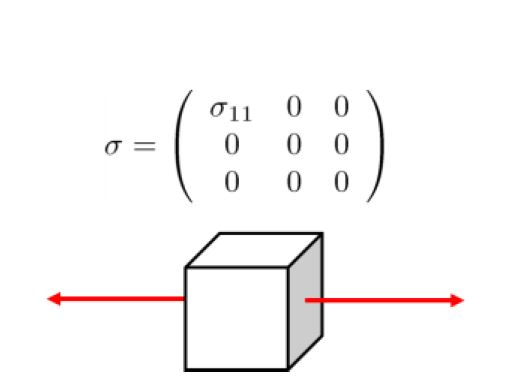
\includegraphics[scale=.12]{images/3Dcfuniaxial}\\
		\hline 
		Plane Stress State && $ \sigma = \begin{pmatrix} \sigma_{11} & \sigma_{12} & 0\\ \sigma_{21} & \sigma_{22} & 0\\ 0 & 0 & 0\\ \end{pmatrix}$&	\vspace*{-1.0cm}	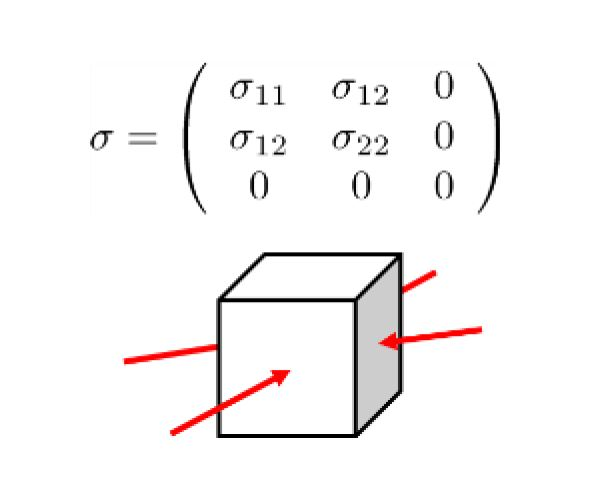
\includegraphics[scale=.12]{images/3Dcfplanestress}\\
		\hline 
		Principal Axis Decompensation &&$ \sigma = \begin{pmatrix} \sigma_{11} &  0& 0\\ 0 & \sigma_{22} & 0\\ 0 & 0 & \sigma_{33}\\ \end{pmatrix}$&\\
		\hline 
		Pure Shear Stress State &$\operatorname{tr}\sigma = 0$&$ \sigma = \begin{pmatrix} 0 &  -s& 0\\ -s & 0 & 0\\ 0 & 0 & 0\\ \end{pmatrix}$&		\vspace*{-1.2cm}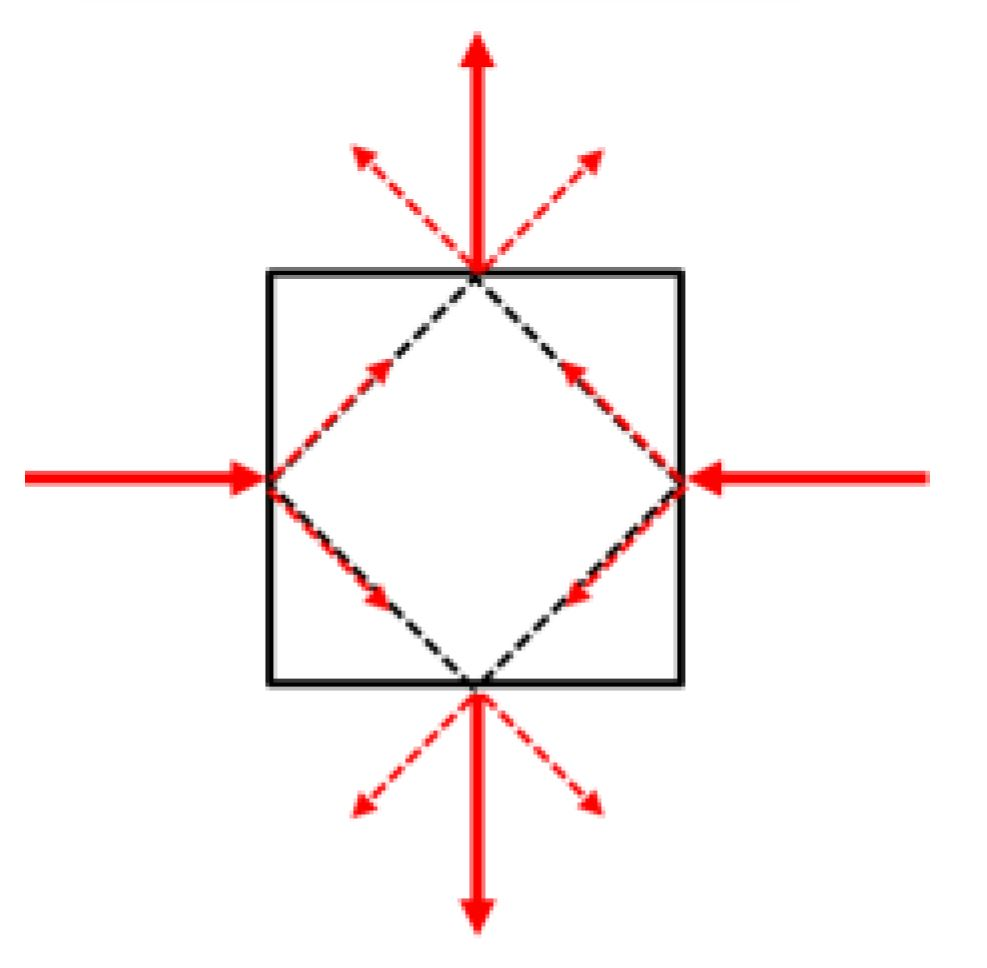
\includegraphics[scale=.12]{images/3Dcfpureshear}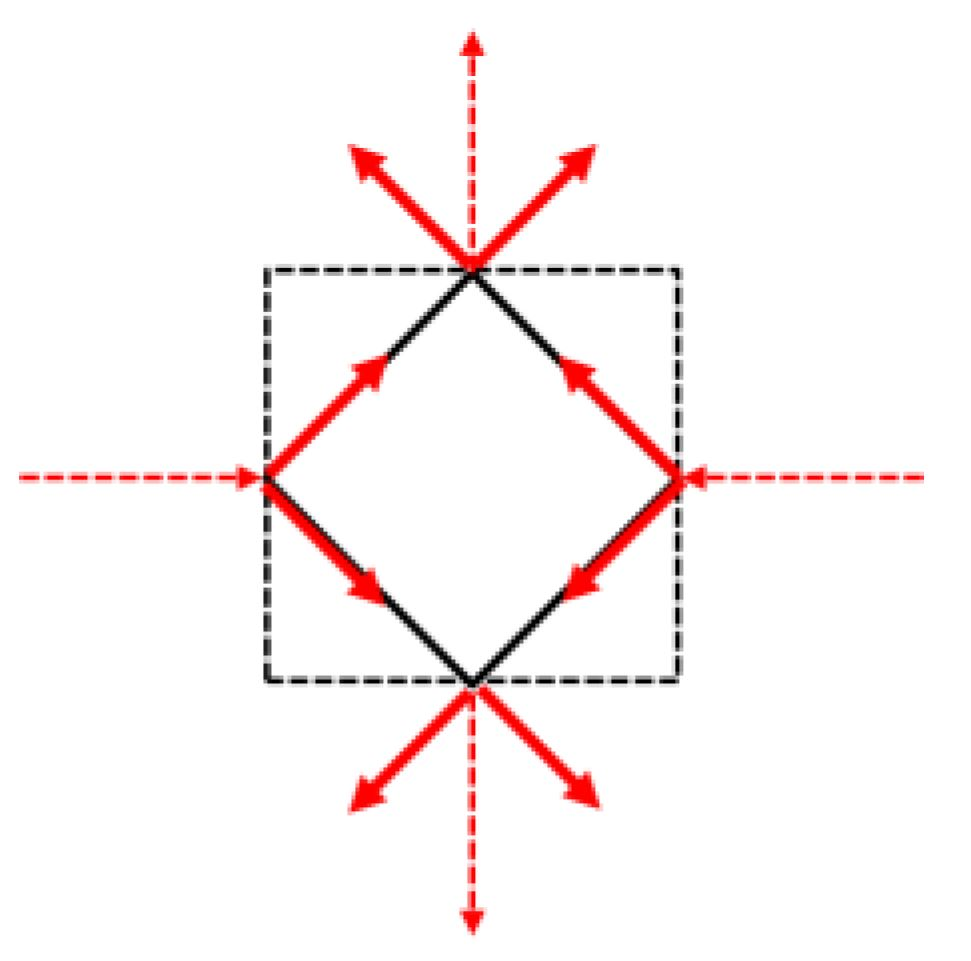
\includegraphics[scale=.12]{images/3Dcfpureshear2}\\
		\hline 
	\end{tabularx}
	\renewcommand{\arraystretch}{1.2}

\subsection{Strain Tensor in 3D}
	Vector of 2nd rank. Gradient of Deformation $u(x)$ \hspace{1cm}$\bm x' = \bm x + \bm u(\bm x)$
	
	\begin{tabularx}{\columnwidth}{p{2cm}XX}
		\hline 
		   $e_{ij} = \dfrac{\partial u_i}{\partial x_j}$&
			$e = \begin{pmatrix}
			\frac{\partial u_1}{\partial x_1} & \frac{\partial u_1}{\partial x_2} &
			\frac{\partial u_1}{\partial x_3}\\
			\frac{\partial u_2}{\partial x_1} & \frac{\partial u_2}{\partial x_2} &
			\frac{\partial u_2}{\partial x_3}\\
			\frac{\partial u_3}{\partial x_1} & \frac{\partial u_3}{\partial x_2} &
			\frac{\partial u_3}{\partial x_3}\\
			\end{pmatrix}$ &
			\vspace*{-.5cm}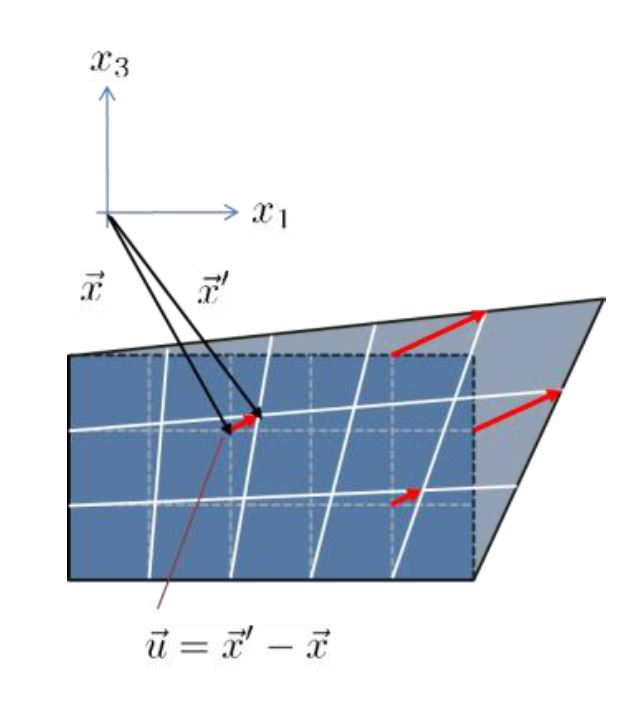
\includegraphics[scale=.2]{images/2Ddeformation}\\
			
			&
			\multicolumn{2}{l}{$\bme = \bme^{sym} + \bme^{anti} = \frac{1}{2}(\bme+\bme^T) + \frac{1}{2}(\bme - \bme^t)$ }\\

			strain tensor & $\varepsilon = \bme^{sym} = \frac{1}{2}(\bme+\bme^T)= \frac{1}{2} (\frac{\partial u_i}{\partial x_j} + \frac{\partial
				u_j}{\partial x_i})$  &\\
			\multicolumn{2}{l}{rotational deformation} & $\gamma = \bme^{anti} = \frac{1}{2}(\bme-\bme^T)$ \\
			\hline
			\multicolumn{3}{c}{\textbf{Rigid body transformation (rigid = starr)}}\\
			\multicolumn{3}{c}{Rigid body transformations do not mechanically deform the body. }\\
			rigid transformation &   
			$x' = x + u(x) \quad u_i(x) = (R_{ij} - \delta_{ij})x_j$ & $R_{ij}$: rotation matrix\\
			&  $\bme \approx \begin{pmatrix} 0 & -\phi &0 \\ \phi &  0& 0 \\  0& 0 & 0\\	\end{pmatrix}$ &
			antimsymmetric deformation tensors correspond to small rotations and don't produce stress within the body\\

			\hline 
			\multicolumn{3}{c}{\textbf{Examples of Strain States}}\\			
			Volume Change of a Deformation & $\dfrac{\Delta V}{V} = \operatorname{tr} \varepsilon$ &
			\vspace*{-.5cm} 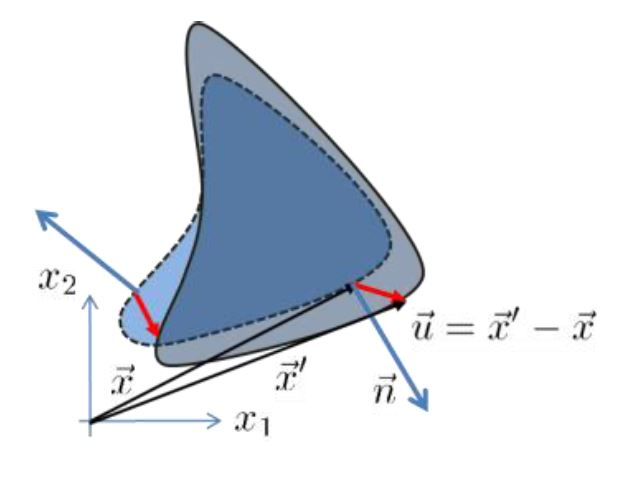
\includegraphics[scale=.2]{images/deformvolume}\\
			\hline 
			pure shear strain & $\operatorname{tr}\varepsilon = 0$ & no volume change\newline only shape chanign\\
			\hline 
			Isotropic Strain &$\varepsilon_{11}=\varepsilon_{22}=\varepsilon_{33}\quad$
			$\varepsilon_{ij} = \varepsilon \cdot \delta_{ij} \qquad \dfrac{\Delta V}{V} = 3\varepsilon_{11}$ & volume changing\newline form of the body stays the same\\
			\hline 
			Plain strain &  $\varepsilon_{33} = \varepsilon_{13} = \varepsilon_{23}= 0$ => $\varepsilon =
				\begin{pmatrix}
				* & * & 0\\
				* & * & 0\\
				* & * & 0\\
				\end{pmatrix} $ &
				No deformation in z axis\\
			\hline 
			Strain Decomposition &   $\varepsilon^{iso}=\frac{\operatorname{tr} \varepsilon}{3} \cdot \mathbb{I} \equiv \frac{1}{3} \mathbb{E} : \varepsilon$&
			$\varepsilon^{shear} = (\mathbb{I} - \frac{1}{3}\mathbb{E}): \varepsilon$\\
			&
			$\varepsilon = \varepsilon^{iso} + \varepsilon^{shear}$ &
			\\
			\hline 

	\end{tabularx}
\newpage
\subsection{Isotropic Mechanical Material Laws}
	\begin{tabularx}{\columnwidth}{p{3cm}XX}
		\hline 
		 \multicolumn{2}{p{10cm}}{$\mathbb{C}^{iso} = K \cdot \mathbb{E} + 2G \cdot (\mathbb{I} - \frac{1}{3}
		 \mathbb{E}) =  (K - \frac{2}{3} G) \cdot \mathbb{E} + 2G \cdot \mathbb{I}$ } &
		 K: bulk modulus(Kompressionsmodul) \newline G: shear modulus(Schubmodul)\\
		 &mostly: $K \gg G$ &\\
		 \hline 
		 \multicolumn{3}{c}{Elasticity Tensor 
		 	$\mathbb{C}^{eng} = K \cdot \begin{pmatrix}
		 		1 & 1 & 1 & 0 & 0 & 0\\
		 		1 & 1 & 1 & 0 & 0 & 0\\
		 		1 & 1 & 1 & 0 & 0 & 0\\
		 		0 & 0 & 0 & 0 & 0 & 0\\
		 		0 & 0 & 0 & 0 & 0 & 0\\
		 		0 & 0 & 0 & 0 & 0 & 0\\
		 	\end{pmatrix}
		 	+ 2 G \cdot \begin{pmatrix}
		 		\frac{2}{3} & -\frac{1}{3} & -\frac{1}{3} & 0 & 0 & 0\\
		 		-\frac{1}{3} & \frac{2}{3} & -\frac{1}{3} & 0 & 0 & 0\\
		 		-\frac{1}{3} & -\frac{1}{3} & \frac{2}{3} & 0 & 0 & 0\\
		 		0 & 0 & 0 & \frac{1}{2} & 0 & 0\\
		 		0 & 0 & 0 & 0 & \frac{1}{2} & 0\\
		 		0 & 0 & 0 & 0 & 0 & \frac{1}{2}\\
		 	\end{pmatrix}$}\\
		 \hline 
		 
		Material reaction to pure compression & $\sigma_{ij}^{comp} = C_{ijkl}^{iso}\varepsilon_{kl}^{comp} = -K\kappa\cdot\delta_{ij}$ & K express material reaction to pure compression\\
		\hline 
		Material reaction to pure Shear Deformation & 
		$\varepsilon_{ij}^{shear} = C_{ijkl}^{iso}\varepsilon_{kl}^{shear} = 2G\varepsilon_{ij}^{shear} $&
		G express material reaction to pure shear compression\\
		\hline 
		Uniaxial stress &
		\multicolumn{2}{p{12cm}}{
		$\begin{pmatrix}
			\sigma_{11}\\
			0\\
			0
		\end{pmatrix} = 
		\begin{pmatrix}
			K + \frac{4G}{3} & K - \frac{2G}{3} & K - \frac{2G}{3}\\
			K - \frac{2G}{3} & K + \frac{4G}{3} & K - \frac{2G}{3}\\
			K - \frac{2G}{3} & K - \frac{2G}{3} & K + \frac{4G}{3}\\
		\end{pmatrix}\cdot
		\begin{pmatrix}
			\varepsilon_{11}\\
			- \varepsilon_{22}\\
			- \varepsilon_{33}
		\end{pmatrix}\qquad
		\sigma_{11} = E\cdot \varepsilon_{11}$ } \\
	\hline 
	Poisson's ration & $\nu = -\dfrac{\varepsilon_{22}}{\varepsilon_{11}} = -\dfrac{\varepsilon_{33}}{\varepsilon_{11}}=\dfrac12 \cdot \dfrac{3K -2G}{3K+G}$&
	ratio of dilation and elongation under uniaxial stress\\
	Young's modulus & $E = \dfrac{\sigma_{11}}{\varepsilon_{11}} = \dfrac{9KG}{3K + G}$&\\
	\hline 
	& \multicolumn{2}{l}{
				$\mathbb{C}^{eng} = \frac{E}{1 + \nu} \cdot \begin{pmatrix}
					\frac{1-\nu}{1-2\nu} & \frac{\nu}{1-2\nu} & \frac{\nu}{1-2\nu} & 0 & 0 & 0\\
					\frac{\nu}{1-2\nu} & \frac{1-\nu}{1-2\nu} & \frac{\nu}{1-2\nu} & 0 & 0 & 0\\
					\frac{\nu}{1-2\nu} & \frac{\nu}{1-2\nu} & \frac{1-\nu}{1-2\nu} & 0 & 0 & 0\\
					0 & 0 & 0 & \frac{1}{2} & 0 & 0\\
					0 & 0 & 0 & 0 & \frac{1}{2} & 0\\
					0 & 0 & 0 & 0 & 0 & \frac{1}{2}\\
				\end{pmatrix}$}\\
		\hline 
	Plane Strain  	 & $\epsilon_{i3} = 0 $\newline damn is an example of such a state& 
	strain Tensor $\varepsilon^{eng} = (\varepsilon_{11}, \varepsilon_{22}, 2\varepsilon_{12})^T$\\
	&$\mathbb{C}^{eng} = \dfrac{E}{1+\nu}\cdot  \begin{pmatrix}
	\dfrac{1-\nu}{1-2\nu} & \dfrac{\nu}{1-2\nu} & 0\\
	\dfrac{\nu}{1-2\nu} & \dfrac{1-\nu}{1-2\nu} & 0\\
	0 & 0 & \dfrac{1}{2}\\
	\end{pmatrix}$&
	$\sigma^{eng} = \mathbb C^{iso,eng}\varepsilon = (\sigma_{11},\sigma_{22}, \sigma_{12})^T$
	\\
	\hline 
	
	Plane Stresss & 
	$\sigma_{i3} = 0$ & 
	\\
	&
	$\mathbb{C}^{eng} = \dfrac{E}{1+\nu}\cdot\begin{pmatrix}
		\dfrac{1}{1-\nu} & \dfrac{\nu}{1-\nu} & 0\\
		\dfrac{\nu}{1-\nu} & \dfrac{1}{1-\nu} & 0\\
		0 & 0 & \dfrac{1}{2}\\
	\end{pmatrix}$
	&\\
	\hline 
	\end{tabularx}


%		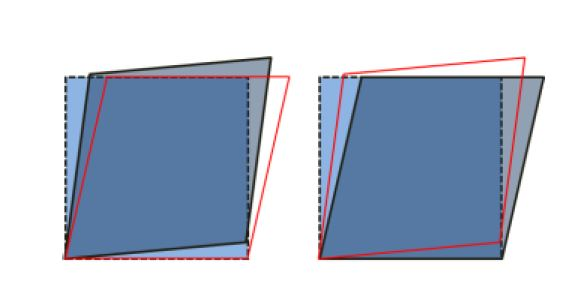
\includegraphics[scale=.3]{images/deformgrad}

%		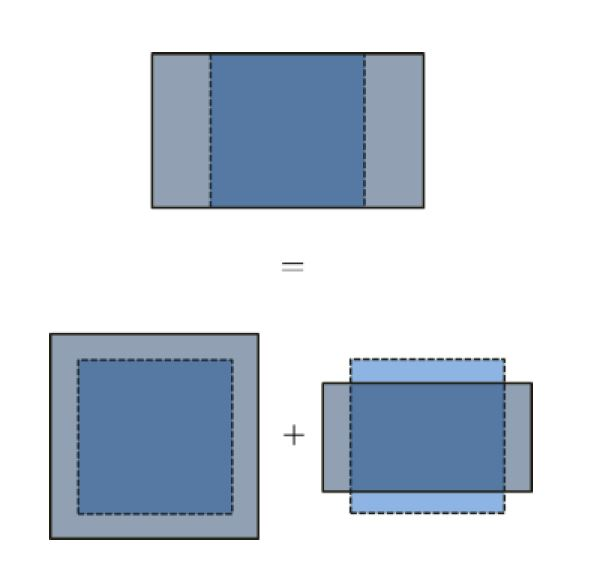
\includegraphics[scale=.3]{images/allstates}
%		\includegraphics[scale=.3]{images/}



